% Le titre de la partie
\section[Back-end]{Simuler une ville ?}

%%%%%%%%%%%%%%%%%%%%%%%%%%%%%%%%%%%%%%%%%%%%%%%%
% Première diapo
%%%%%%%%%%%%%%%%%%%%%%%%%%%%%%%%%%%%%%%%%%%%%%%%

\begin{frame}
	\frametitle{Simuler une ville ?}
	\framesubtitle{Comment simuler avec réalisme et efficacité}

	\begin{alertblock}{Contexte de travail}
	    \begin{itemize}
	        \item Ville à l'échelle de Strasbourg
	        \item 300 000 habitants
        \end{itemize}  
	\end{alertblock}
    
    \onslide<+->{
        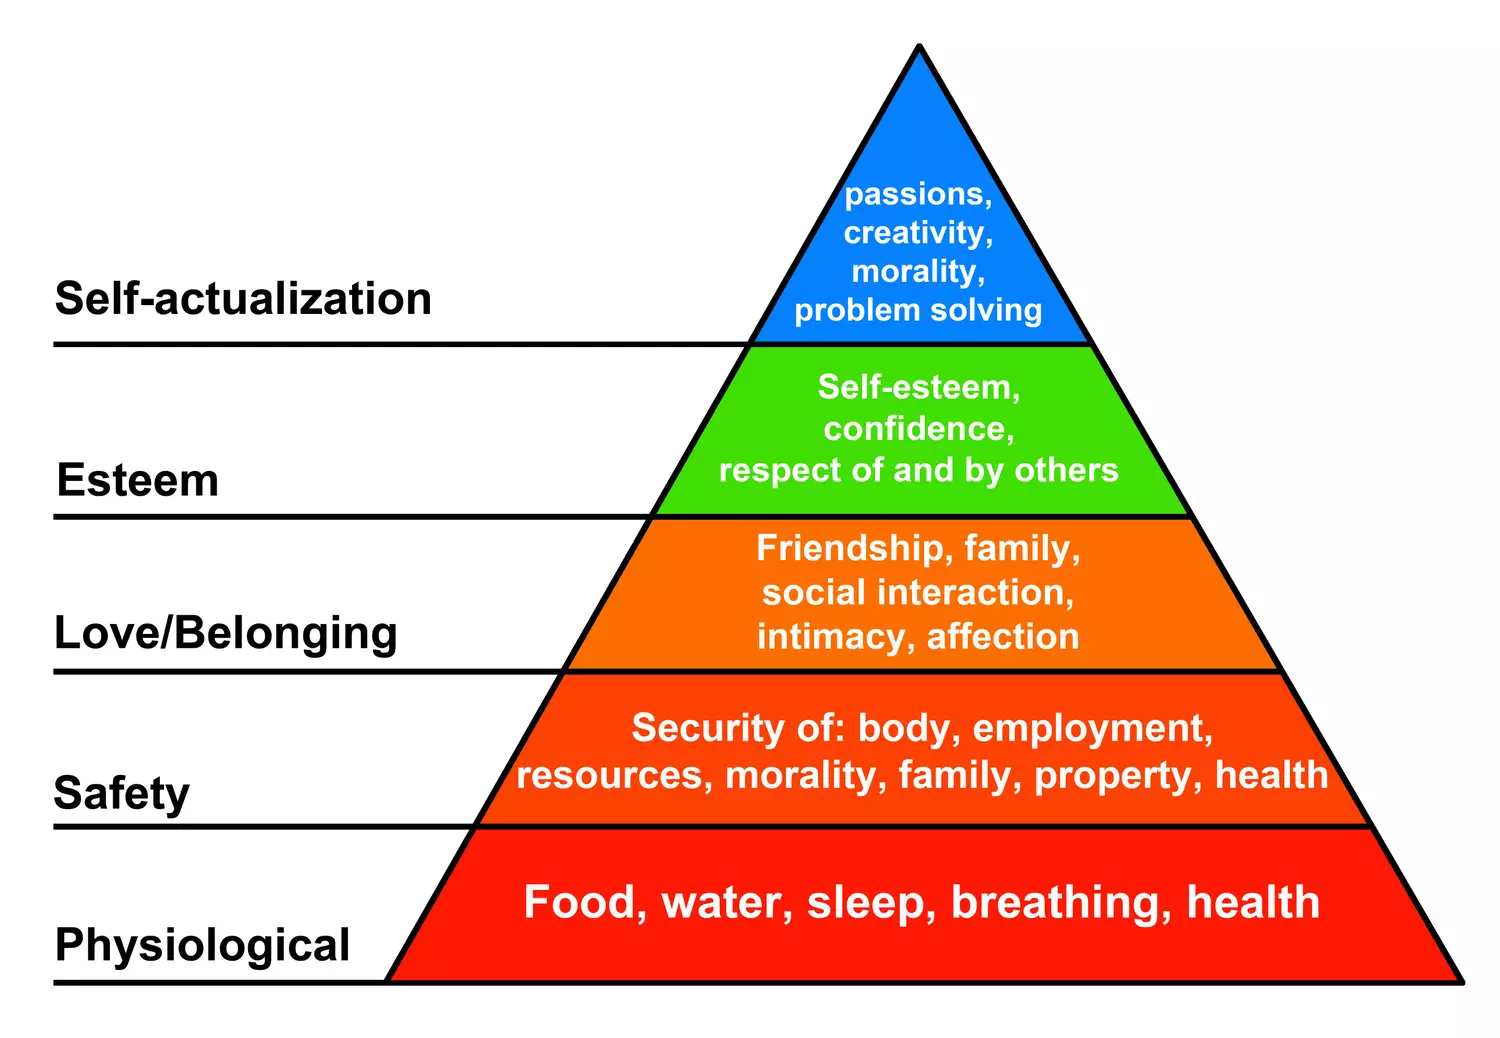
\includegraphics[scale=.1]{diapo/figures/maslow.png}
        $\rightarrow$ étudier la rapidité de réalisation de ces besoins pour chacun.
    }

\end{frame}


\begin{frame}
    \frametitle{Le fonctionnement technique de la simulation}
    \framesubtitle{Que font les citoyens ?}
    
    \begin{center}
        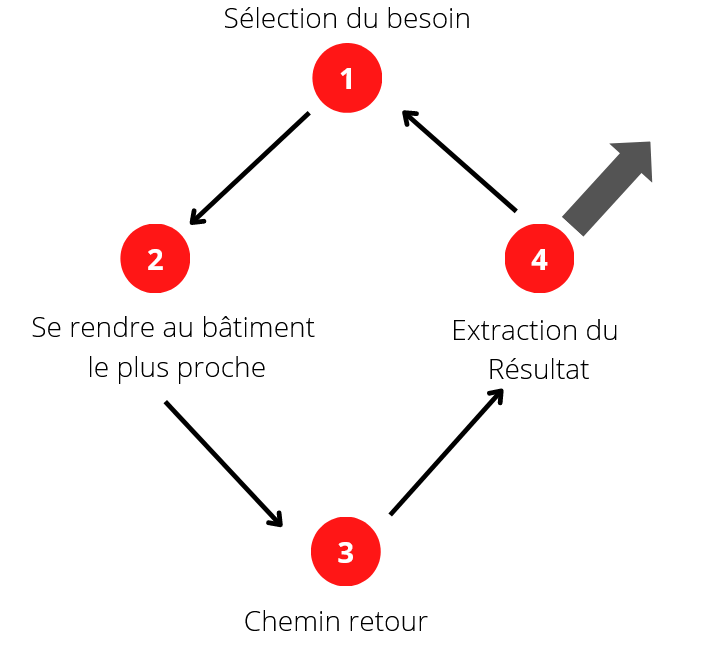
\includegraphics[scale=.3]{diapo/figures/schéma.png}
    \end{center}

\end{frame}


\begin{frame}

    \frametitle{Avancements}
    \framesubtitle{Ca en est où ?}
    
    \begin{center}
        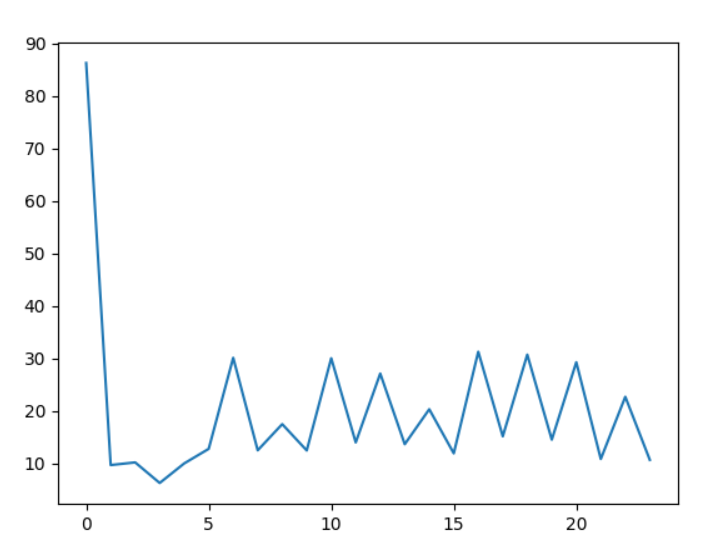
\includegraphics[scale=.25]{diapo/figures/tour.png}\\
        Évolution du temps de tour : très prometteur !
    \end{center}
\end{frame}